\section{Ejercicios IV}


\begin{boxProblem}[fonttitle=\bfseries,title= Cálculo del isomorfismo
$[ \cdot ]_{\beta}: V \longrightarrow \IR^{n}$]
 SSi $V$ es un $F-$espacio vectorial $n-$dimensional y 
$\beta = \{ v_{j} : \hspace{0.2cm} 1 \leq j \leq n \}$
es una base de $V$, entonces, se definió el isomorfismo
\[
[\cdot]_{\beta} : V \longrightarrow F^{n}
\]
como 
\[
T \left( \sum_{j=1}^{n} a_{j} v_{j} \right)
= \begin{pmatrix}
a_{1} \\
a_{2} \\
\vdots \\
a_{n}
\end{pmatrix} \hspace{0.4cm} \textit{ para toda }
x = \sum_{j = 1}^{n} a_{j}v_{j} \in V
\]
Es decir, calcular $[\cdot]_{\beta}$ es lo mismo que expresar 
a un vector arbitrario $x$ de $V$ como combinación lineal de 
elementos de $\beta$
\end{boxProblem}


\marginnote{Si $T: V \longrightarrow V$ es lineal y en $V$ se usa
sólo una base $\beta$, a $[T]_{\beta}^{\beta}$ a veces se le
denota como $[T]_{\beta}$.}
\begin{boxProblem}[fonttitle=\bfseries,title= Cálculo de
representación matricial
$[T]_{\beta}^{\gamma}: V \longrightarrow W$]
SSi $V$ y $W$ son $F-$espacios vectoriales 
finito dimensionales y 
$$\beta = \{ v_{j} : \hspace{0.2cm} 1 \leq j \leq n \} \subseteq V, $$
$$\gamma = \{ w_{k}  | \hspace{0.2cm} 1 \leq k \leq m \} \subseteq W$$
son bases de estos, entonces,
$[T]_{\beta}^{\gamma}$ es una matriz de $m$ filas con $n$ columnas,
donde su $j-$ésima columna es $[T(v_{j})]_{\gamma}$. 

Entonces, $[T]_{\beta}^{\gamma}$ tiene
\begin{itemize}
	\item $n$ columnas, pues hay una por cada elemento de la base $\beta$, y
	\item $m$ filas, ya que cada $T(v_{j})$ necesita $m$ escalares para
	representarse como combinación lineal de elementos de $\gamma$.
\end{itemize}
\end{boxProblem}


Sean 
\begin{equation}
	\label{eq: ej4, beta}
	\beta = \{ (1, 0, 0), (0, 1, 0), (0, 0, 1) \}, 
	\hspace{0.4cm}
	\beta ' = \{ (0, 1, 0), (1, 0, 0), (0, 0, 1) \},
\end{equation}
\marginnote{Nota que $\beta$ y $\beta '$ son iguales como conjuntos,
pero no como bases ordenadas.}
\begin{equation}
	\label{eq: ej4, gamma}
	\gamma = \{ (0, 3, 5), (1, 2, 0), (3, 4, 5) \}, 
	\hspace{0.4cm}
	\gamma ' = \{ (3, 4, 5), (1, 2, 0), (0, 3, 5) \},
\end{equation}

\begin{equation}
\label{eq: ej4, delta}
	\delta = \{ (1, 2, 0), (0, 1, 1), (1, 0, 3) \}.
\end{equation}

\begin{enumerate}
	\item Demuestre que los subconjuntos de $\IR^{3}$ dados en 
	\eqref{eq: ej4, beta}, \eqref{eq: ej4, gamma} y 
	\eqref{eq: ej4, delta} son bases de $\IR^{3}$.
	
	\item Dado $(x, y, z) \in \IR^{3}$ un elemento cualquiera de 
	$\IR^{3}$, expréselo como combinación lineal de elementos
	de las bases del inciso anterior.
	
	\item Dé las fórmulas de los isomorfismos 
	$[ \cdot ]_{\beta}$, $[ \cdot ]_{\gamma}$, 
	$[ \cdot ]_{\delta}$.
	
	\item Sean $T, U : \IR^{3} \longrightarrow \IR^{3}$ las funciones
	\[
	T(x, y, z) = (2x, 5y-z, x+y+z), \hspace{0.4cm}
	U(x, y, z) = (2x+3y, -x, -z+y).
	\]
	Calcule las matrices 
	$[T]_{\beta}^{\gamma}$, $[T]_{\gamma}^{\beta}$, 
	$[T]_{\gamma}^{\delta}$, $[T]_{\delta}^{\gamma}$,
	$[U]_{\beta}^{\delta}$ y $[U]_{\delta}^{\beta}$.
	
	\item Compare a $[T]_{\beta}^{\gamma}$ con $[T]_{\beta '}^{\gamma}$
	y a 
	$[U]_{\beta}^{\gamma}$ con $[T]_{\beta}^{\gamma '}$. ¿Qué relación
	tienen una con otra? ¿Cómo el cambio de orden en una base afecta
	a las matrices?
	
	\item Sea la matriz
	\[
	A = 
	\begin{pmatrix}
	1 & 7 & 0 \\
	0 & 9 & 2 \\
	5 & 1 & 2
	\end{pmatrix} \in M_{3 \times 3} (\IR).
	\]
	Explique por qué existe$^{(*)}$ 
	\marginnote{$(*)$ Pista: usa el teorema fundamental de las bases
	\ref{teo: propiedad univ de las bases}}	
	una única transformación lineal
	$L: \IR^{3} \longrightarrow \IR^{3}$ tal que 
	$[L]_{\beta}^{\gamma} = A$. Encuéntrela.
	
	De igual manera, encuentre a la única transformación lineal
	$S: \IR^{3} \longrightarrow \IR^{3}$ lineal tal que 
	$[S]_{\gamma}^{\delta} = A$. ¿Son $S$ y $L$ iguales?	
\end{enumerate}

Sea 
\begin{equation}
	\label{eq: ejercicio 4 phi}
	\phi = \{ (1, 2), (1, 1) \}.
\end{equation}
\begin{itemize}
	\item Demuestra que $\phi$ es base de $\IR^{2}$.
	\item Da explícitamente al isomorfismo 
	$[\cdot]_{\phi}$.
	\item Sea $K : \IR^{3} \longrightarrow \IR^{2}$
	definida como
	\[
	K(x, y, z) = (2x+z, -y - z).
	\]
	\item Da explícitamente la fórmula de las composiciones
	$K\circ U$ y $K \circ T$.
	\begin{marginfigure}
	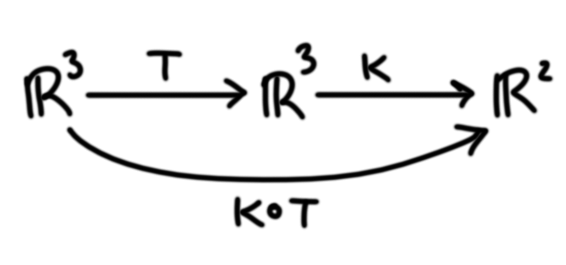
\includegraphics[scale= 1.8]{18} 
	\end{marginfigure}
	\item Usa las fórmulas de estas composiciones para calcular
	las matrices $[K \circ U]_{\delta}^{\phi}$ y 
	$[K \circ T]_{\beta}^{\phi}$.
	\item Calcula las matrices del inciso anterior usando
	representaciones matriciales apropiadas de $T$, $U$ y $K$
	y multiplicándolas entre sí.
\end{itemize}

\textbf{Además,} revisa los ejercicios del capítulo 2.3 del Friedberg,
pero en particular resuelve
3 y 4 de la página 93.
